\subsection{Tikslumo metrikų reikšmės}
\label{subsec:tikslumo_metriku_reiksmes}

Šiame skyrelyje pateikiama gauti apmokyto modelio tikslumo metrikų reikšmės (angl. \textit{accuracy statistics} (žr. \ref{tab:klasifikavimo_metrikos} lentelę).

\begin{table}[H]
    \centering
    \caption{Klasifikavimo tikslumo metrikos.}
    \begin{tabular}{|l|c|c|c|}
        \hline
        \textbf{Metrika} & \textbf{Iris-setosa} & \textbf{Iris-versicolor} & \textbf{Iris-virginica} \\
        \hline
        \textit{True Positives}   & $40$ & $39$ & $40$ \\ \hline
        \textit{False Positives}  & $0$  & $0$  & $1$  \\ \hline
        \textit{True Negatives}   & $80$ & $80$ & $79$ \\ \hline
        \textit{False Negatives}  & $0$  & $1$  & $0$  \\ \hline
        \textit{Recall}           & $1$ & $0{,}975$ & $1$ \\ \hline
        \textit{Precision}        & $1$ & $1$       & $0{,}976$ \\ \hline
        \textit{Sensitivity}      & $1$ & $0{,}975$ & $1$ \\ \hline
        \textit{Specificity}      & $1$ & $1$       & $0{,}988$ \\ \hline
        \textit{F-measure}        & $1$ & $0{,}987$ & $0{,}988$ \\ \hline
    \end{tabular}
    \label{tab:klasifikavimo_metrikos}
\end{table}

Žemiau galima pamatyti (žr. \ref{fig:paklaidos_kitimas_mokymosi_metu} pav.) paklaidos kitimą mokymosi metu.

\begin{figure}[H]
    \centering
    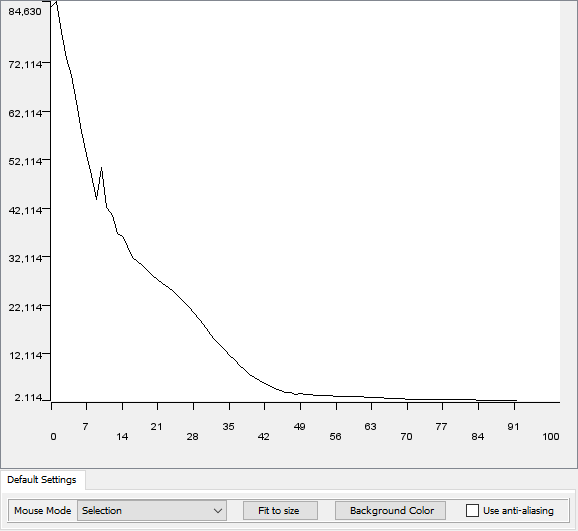
\includegraphics[width=0.85\linewidth]{4Lab/overleaf/images/paklaidos_kitimas_mokymosi_metu.png}
    \caption{Modelio paklaidos kitimas mokymosi metu.}
    \label{fig:paklaidos_kitimas_mokymosi_metu}
\end{figure}

Iš grafiko galima daryti tokias išvadas:
\begin{itemize}
    \item Modelis sėkmingai konvergavo. Paklaida sumažėjo nuo $84{,}63$ iki $2{,}11$
    \item Ties $\sim10$ epocha paklaida šoktelėjo į viršų, bet po to staigiai susitvarkė ir vėl pradėjo mažėti
    \item Nebūtina naudoti $100$ epochų. Jau nuo $\sim50$ epochų paklaida kinta tik minimaliai
\end{itemize}